% !TEX root = ../relatorio.tex

10 filtros passa-faixa de largura $100$ foram desenhados para cobrir o espectro de acordo com a figura \ref{fig:bandas}. Cada filtro for definido com base em sua resposta ao impulso $h[n]=\frac{sin(\omega_{c2}n)-sin(\omega_{c1}n)}{\pi n}$. Os parâmetros $\omega$ foram calculados a partir das frequências pela expressão $\omega = \frac{2f\pi}{f_s}$, que leva a frequência de nyquist para $\pi$, nosso $\omega$ máximo.

\begin{figure}[h]
    \centering
    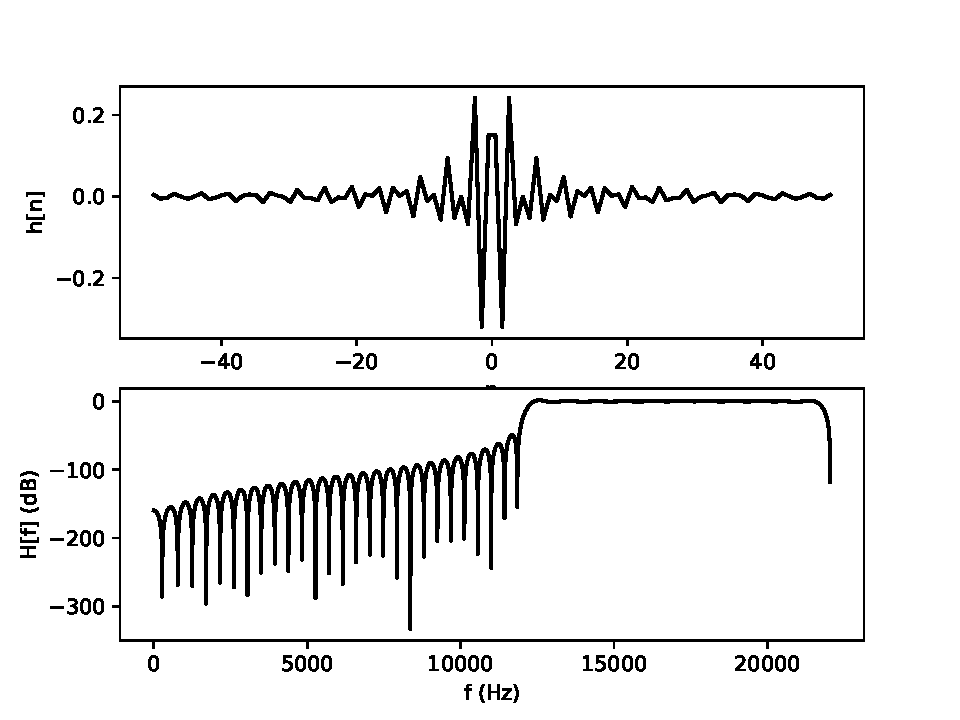
\includegraphics[scale=0.8]{fig/filter9.pdf}
    \caption{Filtro da faixa 12k-22k}
    \label{fig:fnowindow}
\end{figure}

Para "juntar" os filtros, basta somar todas suas representações em resposta impulsiva (coeficientes $a_i$), pois sabemos que $\sum\limits_i^na_ix[n-i]+\sum\limits_i^nb_ix[n-i] = \sum\limits_i^n(a_i+b_i)x[n-i]$.

A resposta impulsiva do filtro resultante da soma de todos os filtros está ilustrada na figura \ref{fig:impulsiva nowindow}.

\begin{figure}[H]
    \centering
    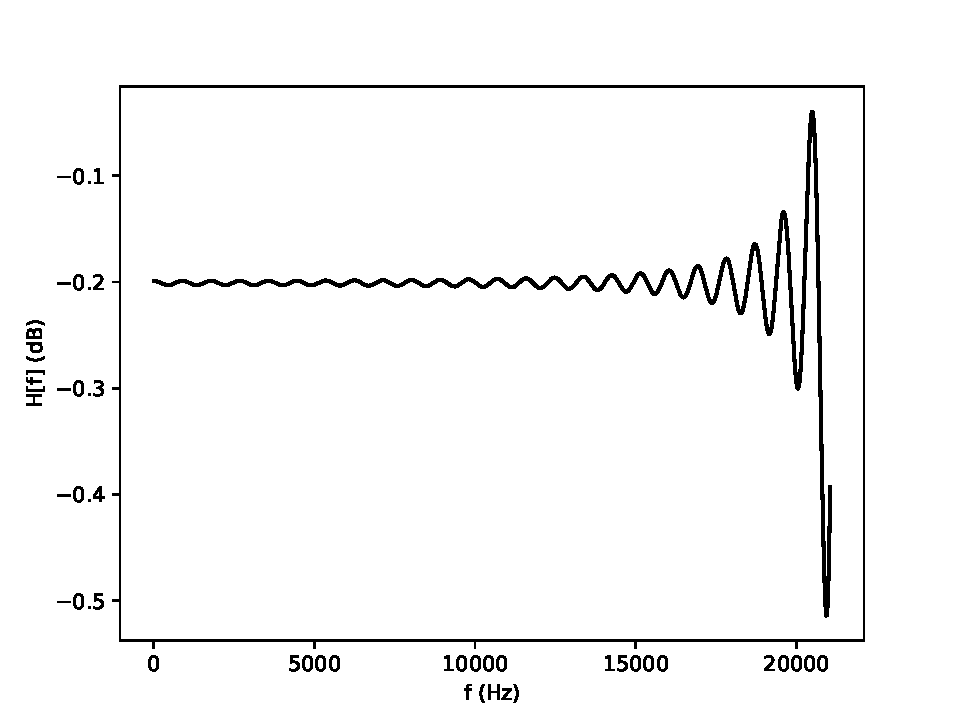
\includegraphics[scale=0.5]{fig/nowindow.pdf}
    \caption{Resposta impulsiva do filtro final sem janelamento}
    \label{fig:impulsiva nowindow}
\end{figure}

Tanto no filtro individual como na resposta impulsiva do filtro final, temos imperfeições indesejáveis provindas da restrição dos filtros a $100$ amostras. Para minimizar esse problema, os filtros foram multiplicados por funções de janelamento.

A função de janelamento utilizada foi uma combinação (multiplicação) da janela de Blackmann-Nuttall (vide equação abaixo) com um janelamento exponencial simples ($e^{k\frac{n}{N}}$).

\[
w[n]=a_0 - a_1 \cos \left ( \frac{2 \pi n}{N} \right)+ a_2 \cos \left ( \frac{4 \pi n}{N} \right)- a_3 \cos \left ( \frac{6 \pi n}{N} \right)
\]
\[
a_0=0.3635819; \quad a_1=0.4891775; \quad a_2=0.
1365995; \quad a_3=0.0106411
\]

A janela resultante é bastante "lisa" (com poucas oscilações) e a redução da resposta em frequência fora da área de interesse é de quase 100dB!

\begin{figure}[H]
    \minipage{0.5\textwidth}
        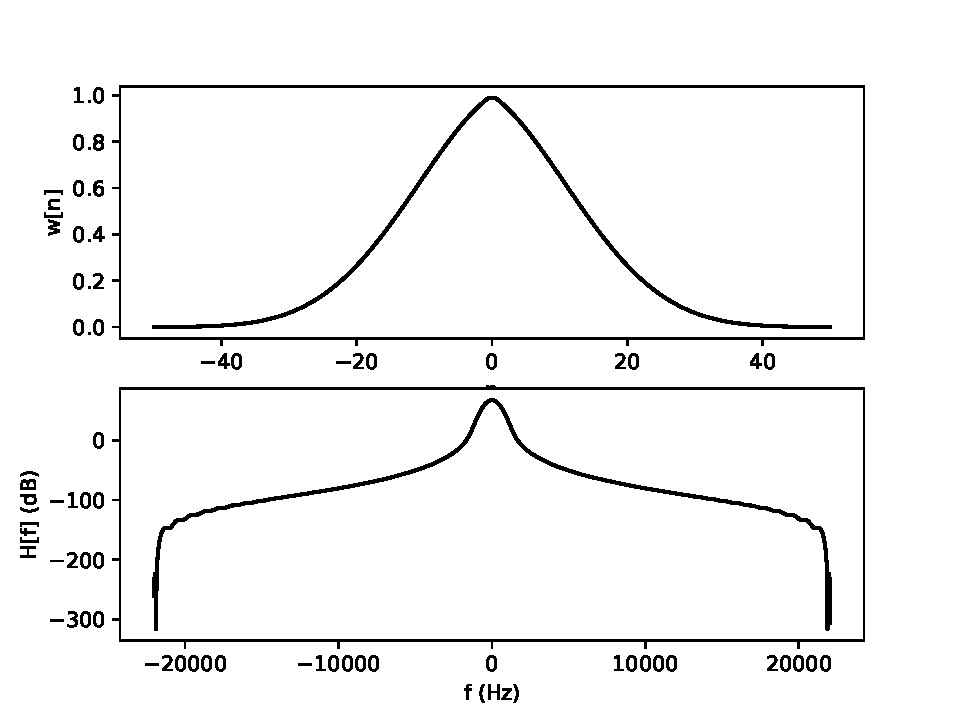
\includegraphics[scale=0.5]{fig/window.pdf}
        \caption{Função de janelamento utilizada}
        \label{fig:window}
    \endminipage
    \minipage{0.5\textwidth}
        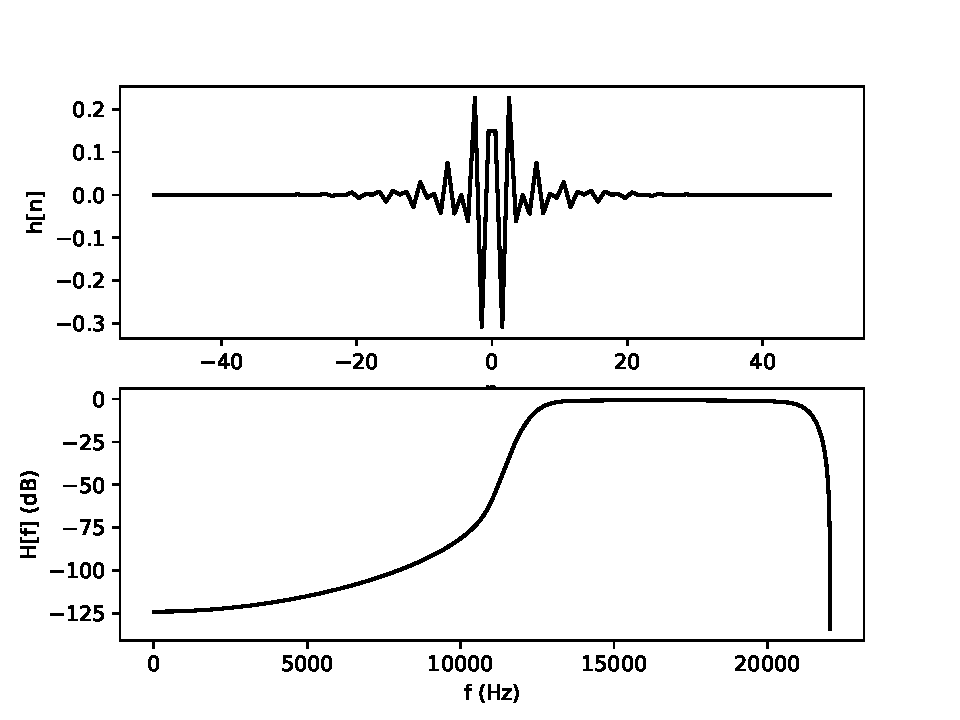
\includegraphics[scale=0.5]{fig/windowfilter9.pdf}
        \caption{Filtro multiplicado pelo janelamento}
        \label{fig:fwindow}
    \endminipage
\end{figure}

A resposta impulsiva resultante dos novos filtros janelados possui bem menos oscilações indesejáveis, como perceptível na figura \ref{fig:impulsiva window}.

\begin{figure}[H]
    \centering
    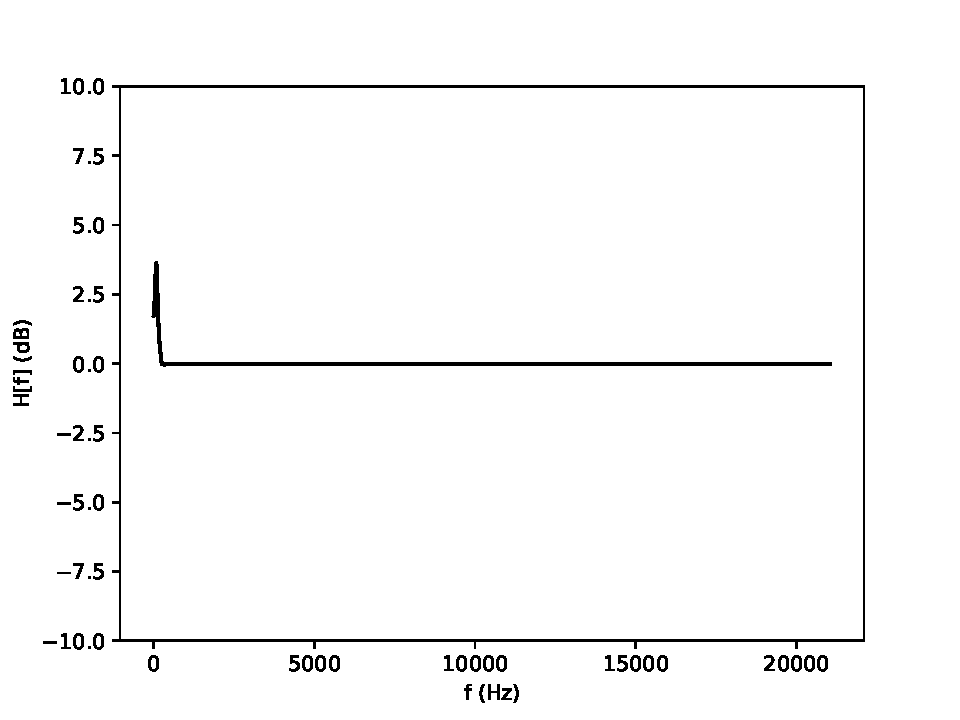
\includegraphics[scale=0.5]{fig/windowed.pdf}
    \caption{Resposta impulsiva do filtro final com janelamento}
    \label{fig:impulsiva window}
\end{figure}

As transições entre bandas do filtro janelado são um pouco menos "bruscas" (\textit{sharp}), mas em compensação, sofrem muito menos com "ringing".

\begin{figure}[H]
    \minipage{0.5\textwidth}
        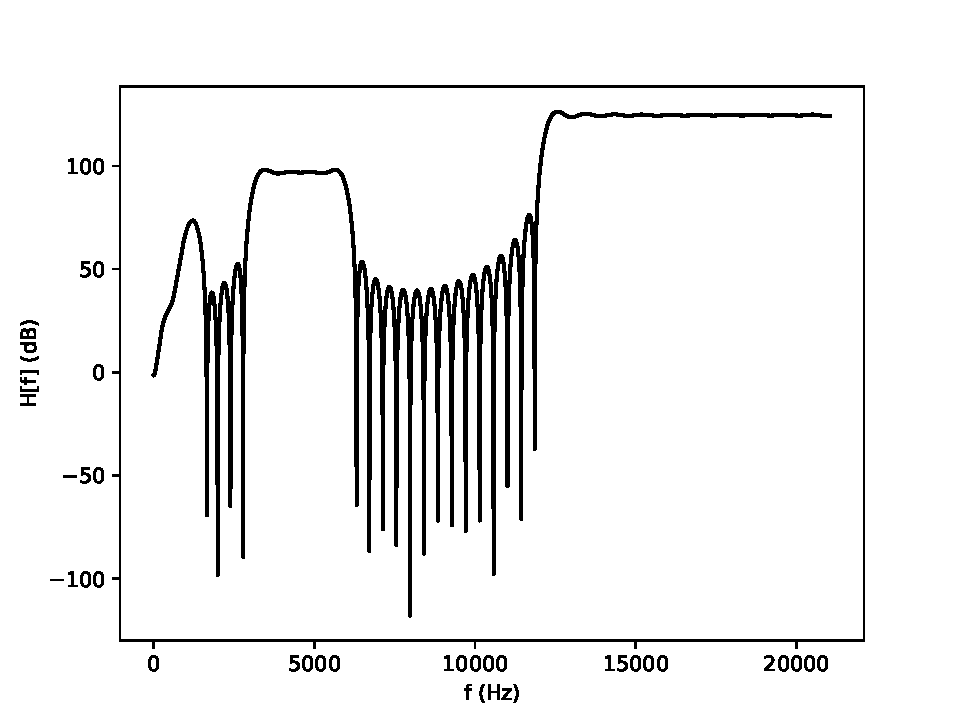
\includegraphics[scale=0.5]{fig/nowindow_stair.pdf}
    \endminipage
    \minipage{0.5\textwidth}
        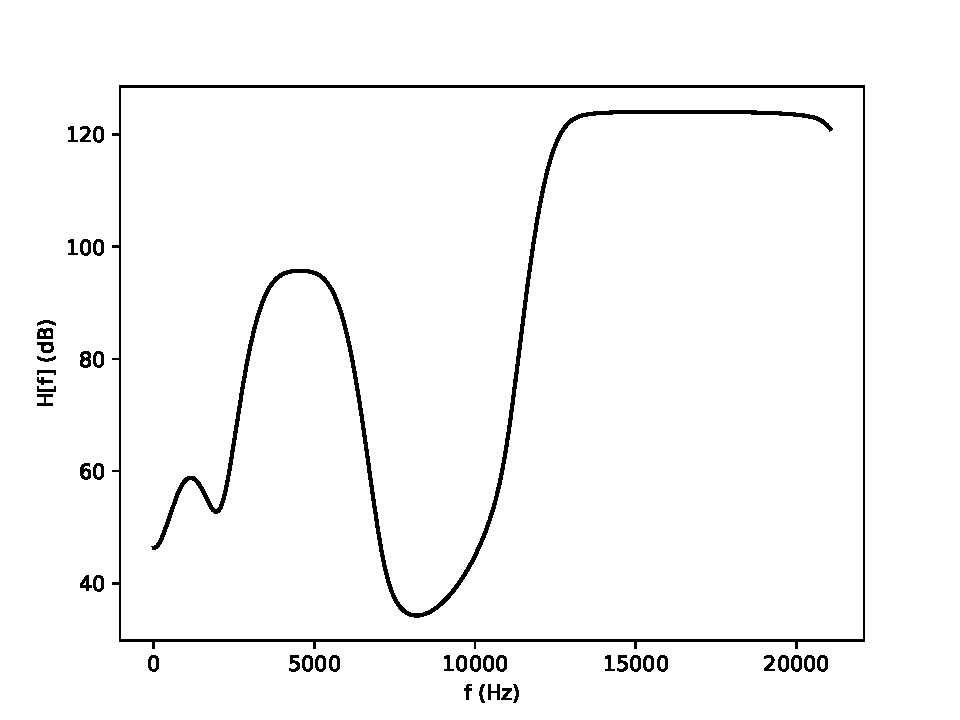
\includegraphics[scale=0.5]{fig/windowed_stair.pdf}
        \endminipage
    \begin{center}
        \caption{Resposta em frequência dos filtros sem e com janelamento}
        \small{(intensificando as bandas ímpares por $2^i$ e atenuando as pares)}
        \label{fig:stair window}
    \end{center}
\end{figure}